\section{Design für Analphabeten}

Beim Design für Analphabeten gibt es einige Ansätze, wie man Dinge wie bspw. Software gestalten kann, damit auch Menschen, die nicht lesen und schreiben können, diese Dinge verwenden können.\\
Hierbei ist es natürlich wichtig herauszufinden, wie diese Menschen Dinge wahrnehmen auffassen und wie ihre Herangehensweise beim erlernen neuer Dinge ist. Um dies herauszufinden ist es unter anderem in erster Linie wichtig Studien abrufen zu können, in denen so etwas bereits gemacht wurde. Dabei muss man in den meisten Fällen jedoch auf Studien zurückgreifen, die sich mit primärem Analphabetismus auseinandersetzen, da diese Studien in den meisten Fällen in Indien und den Phillipinen gemacht wurden, bei Menschen, die das Lesen und Schreiben niemals erlernt haben. Aber auch diese werden voraussichtlich ähnliche Methoden wie funktionale Analphabeten verwenden um zu lernen.\\
Der erste schritt ist sich klar zu machen, dass die Kommunikationsschnittstelle schlecht hin nicht verwendet werden kann. Entsprechend muss das Interface für Analphabeten anders gestaltet werden.

\subsection{Designentwicklung}
Um genau zu bestimmen welche Anforderungen Analphabeten für das Design haben, ist es nötig, dass kontinuierlich mit Probanden zusammen gearbeitet wird. Welche die bisherige Arbeit beurteilen können und den Entwicklern zeigen, an welchen Stellen sie das Design noch nicht soweit getroffen haben, dass ihre Schnittstelle einfach zu verstehen ist. Um zusätzlich zu gewährleisten, das hier ein vernünftiges doch abstraktes Ergebnis erscheint, müssen die Probanden zu jedem Test wechseln und die neuen Probanden müssen es schaffen, sich alleine und ohne Hilfe mit dem ihnen vorliegenden Objekt klar zu kommen. Nur wenn dies geschafft wird, hat man schließlich ein annehmbares Design, welches auch von Leseschwachen verwendet werden kann.\\

Normalerweise wird ein solcher Test mit Dokumente wie Fragebögen oder Aufgabelisten begleitet. 
Dies ist aber bei Analphabeten ein einfach nicht möglich.
Eine Alternative ist die ständige Zusammenarbeit mit dem Probanten, was jedoch zu viel Zeit beansprucht. Eine weitere Alternative ist, die Texte mit Illustrationen oder Audiodateien zu ersetzen oder für funktionale Analphabeten zu erweitern. Ein wichtiges Problem bei der Evaluierung ist das Analphabetismus ihre Schwäche verheimlichen oder ihrer nicht bewusst sind. Dieses verheimlichen führt dazu, dass man nur schwer Probanten findet. Die beste Möglichkeit dabei bietet das Ansprechen von Hilfsorganisationen wie \glqq alphabund\grqq. Über diese Organisationen kann auch leicht auf bereits getätigte Studien zurückgegriffen werden.

\subsection{ Designfolgerungen }
Im Grunde sind die Lösungen für Analphabeten nicht anders als bei \glqq normalen\grqq Benutzern, ausgenommen die Änderungen für primäre und sekundäre Analphabeten. Jedoch sind bei Analphabeten gute Umsetzungen um so wichtiger.\\
Im folgenden werden die Forderungen in vier Kategorien aufgeteilt. 
Die Anforderungen am Lesen beschreiben alle Änderungen, die das lesen der einzelnen Wörter vereinfachen, beziehungsweise ersetzen soll.\\
Die Anforderungen an das Merken beschreiben alle Änderungen, welche den Benutzer konzentrierter Arbeiten lassen.\\
Die Anforderungen an die Metakognition beschreiben die Änderungen, die zum ziehen von Schlüssen hilfreich sind, so zum Beispiel schon das verstehen einzelner Sätze.\\
Zu letzt die Suche und Navigation, welche die Wege beschreiben die der Benutzer verwenden kann.\\\\
Dabei basieren die meisten Schlüsse auf den Fähigkeiten eines Funktionalen Analphabeten, diese können zwar auch mit denen der primären und sekundären Analphabeten arbeiten, doch können durch die semi-textbasierte Anwendung leichter andere Zielgruppen angesprochen werden.

\subsubsection{Lesen}
Welche Möglichkeiten kommen statt Text in Frage? Die naheliegendste Lösung wäre ein Interface, dass die Menschen akustisch anleitet, was zu tun ist, ähnlich der Sehbehinderten. So was ist jedoch manchmal schwierig, denn Audiodateien benötigen viel Speicherplatz und möchte man beispielsweise ein Handy so gestalten, dass auch Analphabeten es benutzen können, so wird der Speicherplatz hier knapp für ein reines Toninterface. Daher sind viele Firmen dazu übergegangen - besonders bei Handys - das Interface mit möglichst wenig Text und mit speziell ausgewählten Bildern zu gestalten, deren Bedeutung leicht zu identifizieren sein soll.\\
Für funktionale Analphabeten lässt sich eingeschränkt auch weiterhin Text verwenden. Dabei sollte Dieser möglichst leicht zu lesen und zu verstehen sein. Dabei sollte man die Schriftart so einfach und lesbar wie möglich gestalten und möglich einheitlich über das ganze Interface sein.\\
Für die Lesbarkeit des Textes ist es wichtig, dass er in einfacher Sprache gehalten ist. Ließt eine Person ein Text die über dem eigenen Verständnis liegt, wird er wesentlich schwerer zu verstehen. Um das zu verdeutlichen kann man die Sprache in verschiedene Schwierigkeitsstufen teilen.
So wäre Stufe 1 das niedrigste Niveau und  12 das von Amtsschriftstücken. Nach einer Studie würden etwa die hälfte aller Amerikaner hier auf Stufe 8 sein. Ein Analphabet liegt in der Regel weit darunter. Verwendet man nun einen Sprachschatz aus der Stufe 8, kommen die normal Benutzer zurecht, verwendet man dann aber zum Beispiel 4 kommen auch die Analphabeten und Möglicherweise auch Kinder zurecht. Das selbe lässt sich auch auf Illustrationen und Audiodateien für andere Gruppen übertragen.

\begin{figure}[h]
	\centering
		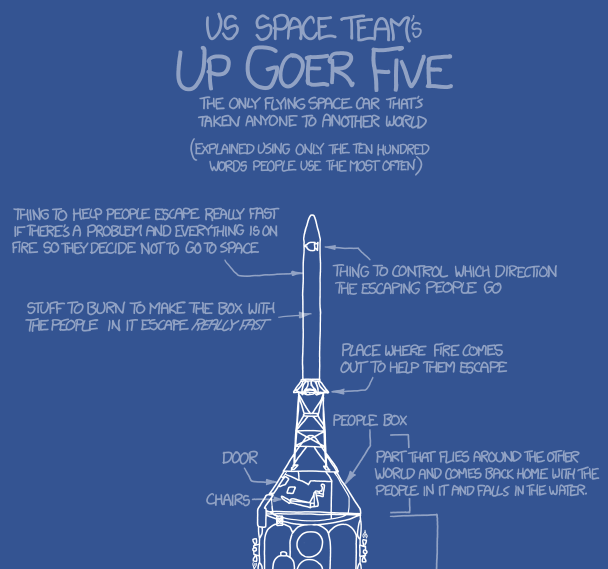
\includegraphics[width=0.50\textwidth]{Daten/up_goer_five_part.png}
	\caption{Up Goer Five: Einfache Sprache aber schwierige Schrift}
	\label{fig:GiveFive}
\end{figure}

\subsubsection{Merken}
Was hat Merken mit Lesen zutun?\\
Direkt nicht viel, außer dass einige Analphabeten auf Grund mentaler Behinderungen nicht lesen können. Jedoch fordert das Merken viel Konzerntration. Vergisst man etwas muss man es erneut lesen und da kommen dann die Schwierigkeiten. Um nun das Merken und somit das Lesen zu unterstützen sollten alle Ablenkungen in der Anwendung entfernt werden. 
Dabei zählt nicht nur blinkende Werbung zu diesen Ablenkungen. Eine der größten Ablenkungen sind andere Aufgaben, die vermieden werden könnten. Denn durch mehrere Aufgaben müssen nicht nur mehr Information gemerkt werden, sondern der Leser muss auch bewerten für was das zu lesende gerade beiträgt. Besonders schwer ist das bei Widersprüchen. Diese zwingen den Benutzer häufig die bereits gelesene Texte erneut zu lesen um den Konflikt zu lösen. Genauso wichtig wie für die üblichen Benutzern sind Informationen besser zu merken und somit auch besser zu verstehen, wenn sie auf die nötigen Informationen reduziert werden. Dazu eignet es sich die Informationen in sich geschlossene Abschnitte einzuteilen.

\subsubsection{Metakognition}
Die Metakognition ist dem Merken und Lesen sehr ähnlich, da sie hier mit dem kombinieren oder auch verstehen des Gemerkten als Ganzes zu verstehen ist. Dabei wird der Benutzter meist mehr auf sich verlassen als nötig. So kann man die derzeitigen Ziele wie zum Beispiel Anmelden und Thema auswählen Angeben. Am sinnvollsten sollten diese in der Form einer Checkliste immer ersichtlich sein. Auch können Wahlmöglichkeiten zu Problemen führen, da der Benutzer erst einmal die einzelnen Möglichkeiten unterscheiden muss. So kann der Benutzer jeder Zeit schauen, was er gerade machen muss, was er gemacht hat und was noch kommt. Genauso wie so die Aufgaben einheitlich dargestellt werden sollten, sollte auch das restliche Design einheitlich und konsistent sein. Damit kann er die bereits bekannten Schaltflächen schneller verwenden.\\
\begin{figure}[h]
	\centering
		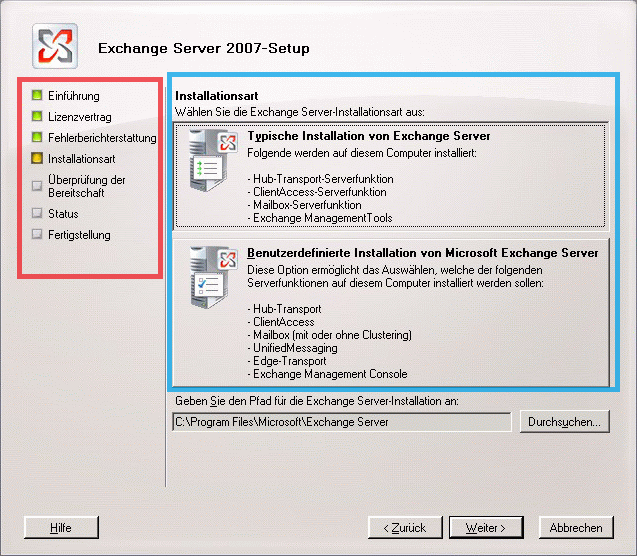
\includegraphics[width=1.00\textwidth]{Daten/ServerBeispiel.png}
	\caption{Interface mit Checkliste und Wahlmöglichkeiten}
	\label{fig:InstallBsp}
\end{figure}

\subsubsection{Navigation und Suche}
Übersicht ist für jeden Benutzer sinnvoll. Jedoch ist es schwer die Balance zwischen vielen Wahlmöglichkeiten und der Tiefe der Wahlmöglichkeiten zu finden. Gerade beim unterscheiden der Alternativen sollte klar sein, wo was hinführt. Dabei wird das gerade für Analphabeten schnell unübersichtlich und die Möglichkeiten sollten gering gehalten werden. Jedoch fühlen sich Analphabeten auch schneller verloren und somit sollten die Suchwege nicht zu lang werden. Um diesen Konflikt etwas aufzulösen bietet sich das Anzeigen des Verlaufs an. Ebenso sollten die wichtigsten oder auch häufigsten Inhalte wie Suche, Anmelden und Hilfe möglichst ohne suchen zugänglich sein. Der Analphabetismus stellt gerade für die Suche eine Herausforderung dar, da der Benutzer die Wörter mit denen er sucht meist nicht richtig schreiben kann. Die Suche muss somit die Wörter interpretieren was sie entsprechen könnten.
\begin{figure}[h]
	\centering
		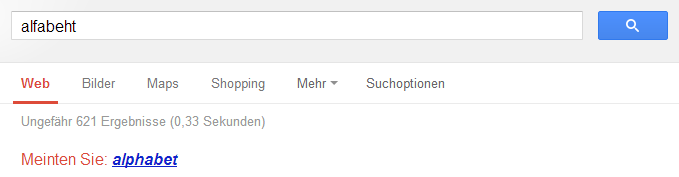
\includegraphics[width=0.80\textwidth]{Daten/rechtschreibung.png}
	\caption{Fehlerkorrektur der Suche bei Google}
	\label{fig:GoogleSearch}
\end{figure}

\subsection{Beispiele: Design für Analphabeten}

Nun wollen wir ein paar Beispiele nennen, in denen man sich mit genau diesem Problem beschäftigt hat und entsprechende Lösung dafür für die Öffentlichkeit bereithält (Abb \ref{fig:DesignBeispiel1}).

\subsubsection{Auditives Text-Design}

\begin{figure}[h]
	\centering
		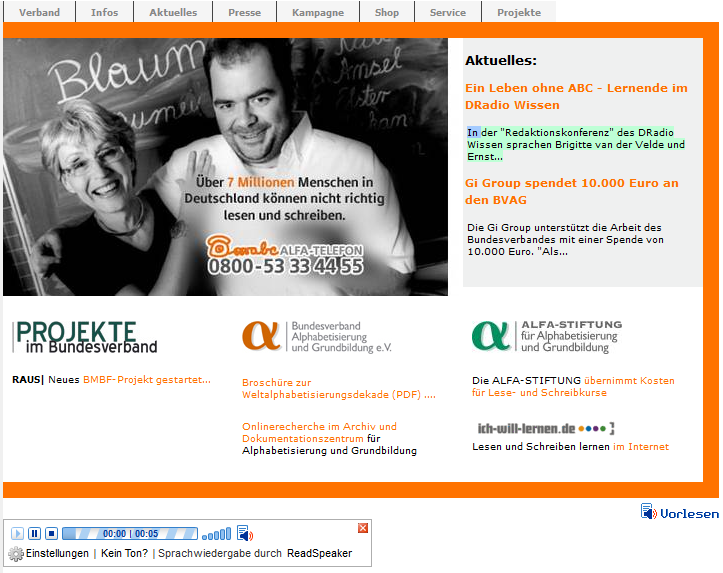
\includegraphics[width=0.80\textwidth]{Daten/DesignBeispiel1.png}
	\caption{Design Beispiel vom Bundesverband Alphabetisierung}
	\label{fig:DesignBeispiel1}
\end{figure}

Hier kann man auf Abb.\ref{fig:DesignBeispiel1} einen markierten Text sehen und unten rechts einen kleinen Button, auf dem "`Vorlesen"' steht. Diese Anwendung ist so gedacht, dass sobald User einen Text markieren, diese den Vorschlag eingeblendet bekommen, dass ihnen dieser Text doch einfach vorgelesen werden könnte. Ohne Zweifel ein Design, dass sich in erster Linie bestenfalls für funktionale Analphabeten auszahlt, oder zumindest für Leute, die eine kurze Einführung erhalten. Jedoch ist die Idee, die hinter dem ganzen steckt eine Fantastische, die dem User eine Möglichkeit anbietet schwierigen Text für ihn zu entziffern, wenn er dazu nicht in der Lage ist. Akkustisch fällt schlimmstenfalls noch das Problem ins Gewicht, dass Worte vielleicht unbekannt sein könnten, aber dies wollen wir hier nicht näher behandeln.\\
Der User kann sich in so wie man es sieht, wirklich jeden Text markieren - ausgenommen natürlich den Text auf Bildern - und ihn sich vorlesen lassen, wodurch er sogar eine Möglichkeit hat, sich die Navigation an der Stirnseite der Seite vorlesen zu lassen. Wenn man also erst einmal weiß, wie man in etwa mit einer Maus umgeht, kann sich jeder User, der dieser Sprache mächtig ist über die ganze Seite navigieren lassen und sich immer anhören, was die Maschine zu sagen hat, wenn er selber es nicht schafft.\\
\newpage
\subsubsection{Reines Text-Design}

Es gibt auch andere Varianten, die reinweg für funktionale Analphabeten gedacht sind. In diesem Punkt kommen wir nun zu der Suchmaschine Invisque (INteractive VIsual Search and QUery Environment). Diese Suchmaschine ist in erster Linie nicht nur für Analphabeten entwickelt worden, aber wurde laut Angaben der Entwickler so weiterentwickelt, dass sie auch für funktionale Analphabeten geeignet sein soll. Um dieses Ziel zu erreichen, haben die Entwickler versucht einigen Problemen, die funktionale Analphabeten haben, entgegen zu wirken, wie das es diesen Menschen schwer fällt sich auf den Text zu konzentrieren, wenn sehr viel ablenkender weiterer Text auf der Seite verteilt wird, oder wenn PopUps auftauchen, oder Werbung allgemein an den Rändern blinkt. All dies blendet Invisque erfolgreich aus mit einer Blanko-Oberfläche. Invisque verwendet einen wenig irritierenden weißen Hintergrund, in den Ecken befinden sich kleine Felder, aus denen man sich weitere Informationen und Navigationsunterstützung besorgen kann. wie auf Abb.\ref{fig:Invisque} zu sehen ist.


\begin{figure}[h]
	\centering
		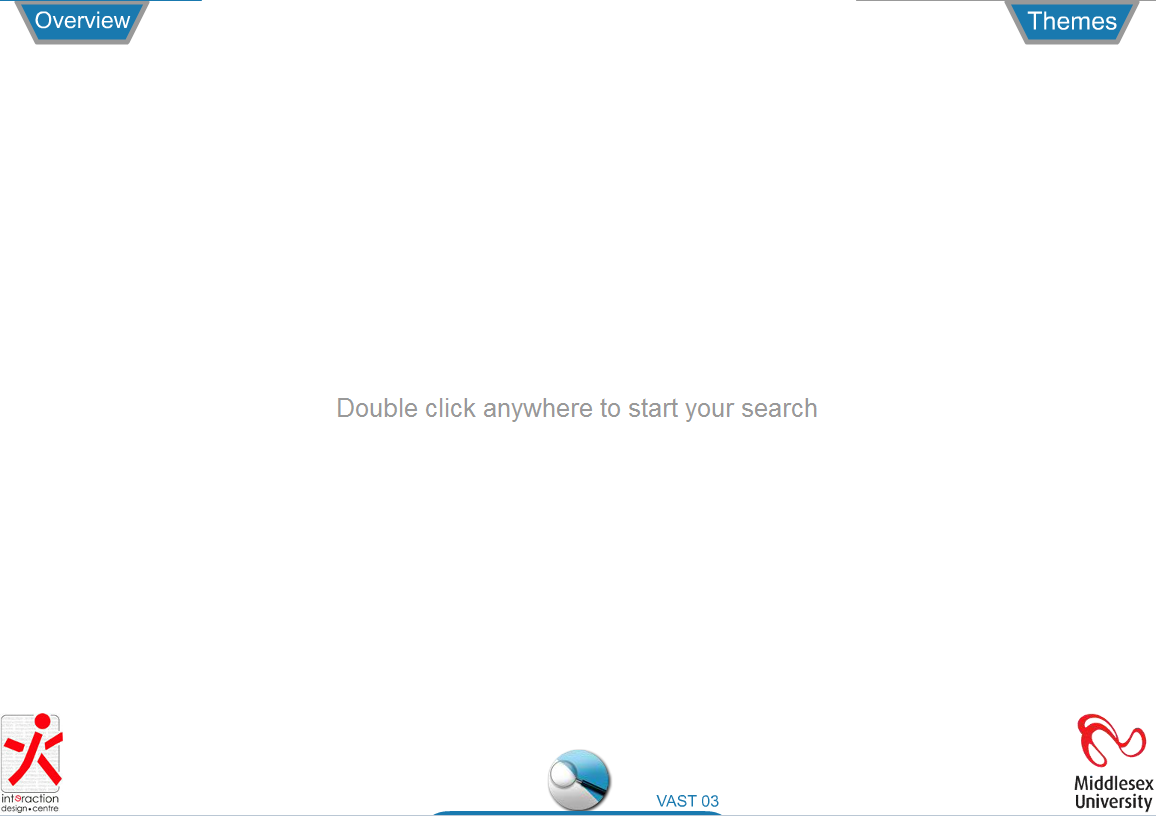
\includegraphics[width=0.80\textwidth]{Daten/Inisque.PNG}
	\caption{Invisque Oberfläche}
	\label{fig:Invisque}
\end{figure}

Um einen guten Überblick über diese Suchmaschine zu bekommen, kann man nur empfehlen, es selber ein wenig auszuprobieren und verschiedene Schlüsselwörter einzugeben, mit denen man sich mit der Suche vertraut macht.

\subsubsection{Ein reines Bild Design}

Ein weiterer Ansatz ist es, den Analphabeten ein Interface zu liefern, in dem diese nur über Bilder gezeigt bekommen, worum es geht. Dies ist sicherlich für die Entwicklung eine große Herausforderung, da nicht jeder Mensch Bilder auf die gleiche Weise interpretiert, daher muss darauf geachtet werden, dass die Bilder absolut eindeutig in einem entsprechenden Kontext zugeordnet werden können. Ein Beispiel sind die Bilder für die Tätigkeiten aus der nachfolgenden Anwendung. Hier mussten Details wie fließendes Wasser oder Feuer hinzugefügt werden um zuverdeutlichen, dass es sich um spülen und kochen handelt.

\begin{figure}[h]
	\centering
		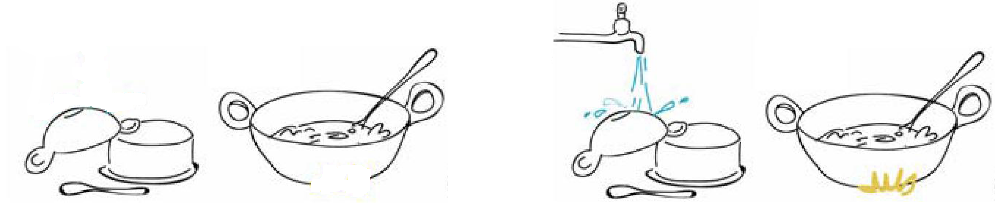
\includegraphics[width=1.00\textwidth]{Daten/pic_fail2.PNG}
	\caption{Deutlichkeit der Illustrationen}
	\label{fig:picfail}
\end{figure}

Bei diesem Design handelt es sich um eine Anwendung, welche allen Arten von Analphabeten dabei helfen soll, einen neuen Job zu finden. Diese spezielle Anwendung wurde in Indien entwickelt und speziell für Menschen aus Slums programmiert. Der Grund und die Inspiration für diese Software war, dass es dort viele Menschen gibt, die wenn sie einen Job haben, diesen nicht mehr aufgeben, auch wenn der Lohn, den sie dafür erhalten viel zu niedrig ist und sie die Chance hätten, einen besseren Job zu bekommen.\\
Das Problem dieser Leute hier, ist was man natürlich an dieser Stelle nicht vergessen darf, dass sie nicht lesen können und entsprechend, nicht über Jobangebote informiert werden. zudem geht es hierbei auch noch um Menschen, die in den Slums wohnen und dadurch besonders wenig Anschluss an die restliche Gesellschaft und keinerlei Erfahrung mit dem Umgang mit digitaler Technik haben. Daher wollte man diese Software entwickeln um genau diesen Menschen zu helfen, ihre Lebensqualität ein wenig zu verbessern.\\
Um schon mal einen direkten Eindruck von der Applikation zu bekommen, betrachte man bitte Abb.\ref{fig:joblist}.


\begin{figure}[h]
	\centering
		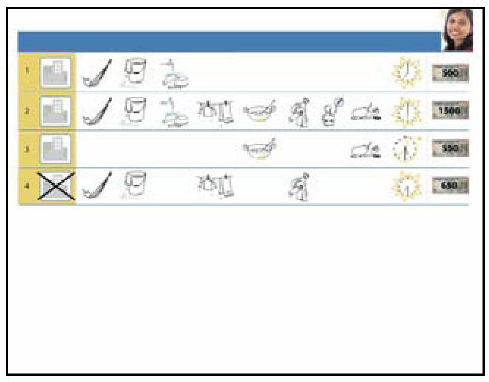
\includegraphics[width=0.90\textwidth]{Daten/job_list.PNG}
	\caption{Job Liste basierend auf Bildern}
	\label{fig:joblist}
\end{figure}

Man sieht, die Anwendung besteht wie versprochen nur aus Bildern. Was wir hier sehen, ist eine Liste von Jobs, wobei die Bilder die Beschreibung zu dem liefern, was getan werden soll, wie Fegen oder Kochen. Rechts sind noch eine Uhr abgebildet, die den Menschen sagt, wann sie beginnen müssen zu arbeiten - nähere Informationen, wie wie lange sie arbeiten müssen, erhalten sie, wenn sie diese Job anklicken und damit zu den ausführlicheren Informationen gelangen - und daneben einen Geldschein mit einer Zahl drauf, der ihnen sagt, wie viel sie dort verdienen können.\\\\
In der Abb. \ref{fig:jobclose} werden nun alle Informationen detailierter gestaltet. Die Uhrzeiten werden in der allerseits bekannten analogen Form dargestellt. Vormittags und Nachmittags wird über eine Sonne, bzw. Mond verdeutlicht. Falls die Zahlen doch nicht gelesen werden können, findet sich hier rechts die korrekte Anzahl der Geldscheine.\\\\

Eine weiteres auf Bildern Basierendes Design ist in Abb. \ref{fig:mapsimple} zu sehen.
Hier wollte man der selben Zielgruppe helfen sich leichter zurecht zufinden. Da normale Karten für Analphabeten, Aufgrund dem Focus auf Straßenanmen nicht lesbar sind. Statt Straßennamen werden hier nun Merkmale zur orientierung genutzt. So sind vorallem Krankenhäuser und andere Auffällige Gebäude angegeben.
\begin{figure}[h]
	\centering
		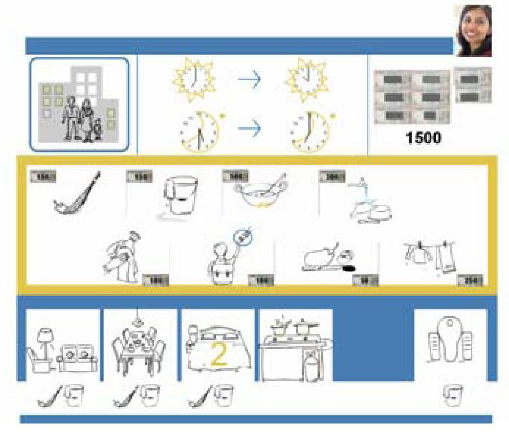
\includegraphics[width=0.8\textwidth]{Daten/job_close.PNG}
	\caption{Job Ansicht}
	\label{fig:jobclose}
\end{figure}

\begin{figure}[h]
	\centering
		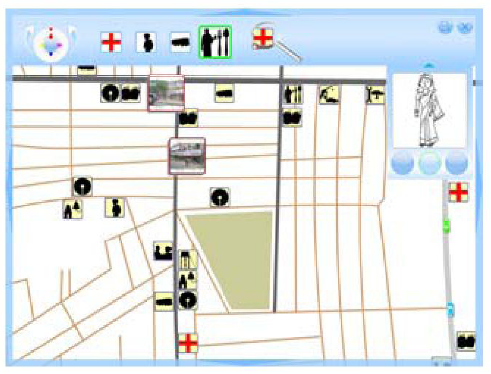
\includegraphics[width=0.8\textwidth]{Daten/map_simple.PNG}
	\caption{Job Liste basierend auf Bildern}
	\label{fig:mapsimple}
\end{figure}
\clearpage